
% {\setbeamercolor{background canvas}{bg=red!15}

\begin{frame}[fragile]
\frametitle{Challenge: Font Styles}
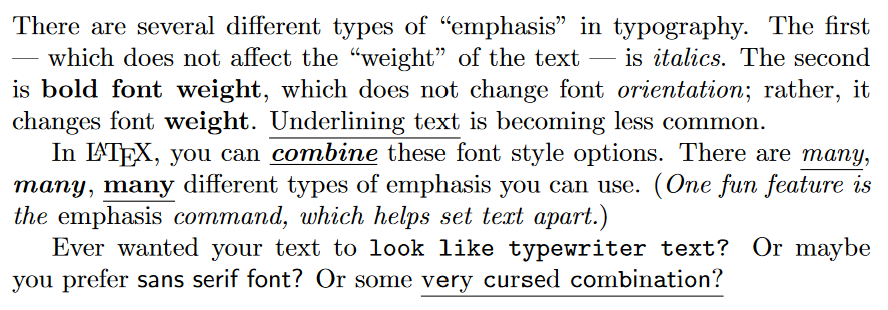
\includegraphics[width=\linewidth]{img/FontEmphs.png}
\end{frame}


\begin{frame}[fragile]
\frametitle{Challenge: Font Styles}
\begin{alertblock}{Font Styles: Source Code (1/3)}
\small
\begin{minted}{latex}
There are several different types of ``emphasis" in 
typography.
The first --- which does not affect the ``weight" of the
text --- is \textit{italics}.
The second is \textbf{bold font weight}, which does not 
change font \textit{orientation}; rather, it changes font
\textbf{weight}.
\underline{Underlining text} is becoming less common.
\end{minted} 
\end{alertblock}
\end{frame}


\begin{frame}[fragile]
\frametitle{Challenge: Font Styles}
\begin{alertblock}{Font Styles: Source Code (2/3)}
\small
\begin{minted}{latex}
In \LaTeX{}, you can \textit{\textbf{\underline{combine}}}
these font style options. 
There are \textit{\underline{many}}, 
\textbf{\textit{many}}, \textbf{\underline{many}} 
different types of emphasis you can use. 
(\textit{One fun feature is the \emph{emphasis} command, 
which helps set text apart.})
\end{minted} 
\end{alertblock}
\end{frame}


\begin{frame}[fragile]
\frametitle{Challenge: Font Styles}
\begin{alertblock}{Font Styles: Source Code (3/3)}
\small
\begin{minted}{latex}
Ever wanted your text to \texttt{look like typewriter 
text?} Or maybe you prefer \textsf{sans serif font?} Or
some \underline{\textrm{v}\texttt{e}\textsf{r}\textrm{y} 
\texttt{c}\textsf{u}\textrm{r}\texttt{s}\textsf{e}
\textrm{d} \texttt{c}\textsf{o}\textrm{m}\texttt{b}
\textsf{i}\textrm{n}\texttt{a}\textsf{t}\textrm{i}
\texttt{o}\textsf{n}\textrm{?}}
\end{minted}
\end{alertblock}
\end{frame}


\begin{frame}[fragile]
\frametitle{Exercise: Font Colors}
Add the following line to the preamble of your document. \\
\textit{\small Try to keep the preamble structured logically!}
\begin{alertblock}{}
\small
\begin{minted}{latex}
\usepackage{xcolor}   
\end{minted}
\end{alertblock}
\end{frame}


\begin{frame}[fragile]
\frametitle{Challenge: Font Colors}
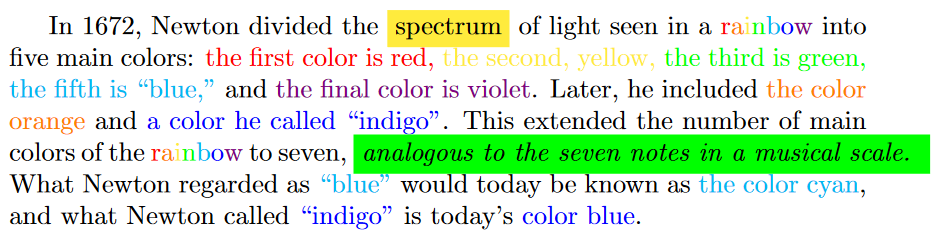
\includegraphics[width=\linewidth]{img/colorsChallenge.png}
\end{frame}


\begin{frame}[fragile]
\frametitle{Challenge: Font Colors}
\begin{alertblock}{Font Colors: Source Code (1/2)}
\small
\begin{minted}{latex}
In 1672, Newton divided the \colorbox{yellow}{spectrum} of 
light seen in a \textcolor{red}{r}\textcolor{orange}
{a}\textcolor{yellow}{i}\textcolor{green}
{n}\textcolor{cyan}{b}\textcolor{blue}
{o}\textcolor{violet}{w} into five main colors: 
\textcolor{red}{the first color is red,} 
\textcolor{yellow}{the second, yellow,} 
\textcolor{green}{the third is green,} 
\textcolor{cyan}{the fifth is ``blue,"} and 
\textcolor{violet}{the final color is violet}.
Later, he included \textcolor{orange}{the color orange} 
and \textcolor{blue}{a color he called ``indigo"}. 
\end{minted} 
\end{alertblock}
\end{frame}

\begin{frame}[fragile]
\frametitle{Challenge: Font Colors}
\begin{alertblock}{Font Colors: Source Code (2/2)}
\small
\begin{minted}{latex}
This extended the number of main colors of the 
\textcolor{red}{r}\textcolor{orange}{a} 
\textcolor{yellow}{i}\textcolor{green}{n} 
\textcolor{cyan}{b}\textcolor{blue}{o} 
\textcolor{violet}{w} to seven, \colorbox{green}
{\textit{analogous to the seven notes in a musical scale.}}
What Newton regarded as \textcolor{cyan}{``blue"} would 
today be known as \textcolor{cyan}{the color cyan}, and 
what Newton called \textcolor{blue}{``indigo"} is today's  
\textcolor{blue}{color blue}.
\end{minted} 
\end{alertblock}
\end{frame}



% }
